% \section{Algorithms}
\section{Communication-Efficient Triangle Counting Algorithms}
% \section{Two-Rounds Local Triangle Algorithms}
\label{chap2-sec:algorithms}
The current state-of-the-art triangle counting algorithm~\cite{Imola_USENIX21} under edge LDP suffers from an extremely large per-user download cost; 
% hence 
% and therefore 
% is impractical for a large graph. 
e.g., every user has to download a message of $400$ Gbits or more when $n=900000$. 
Therefore, it is impractical for a large graph. 
To address this issue, we propose three communication-efficient triangle algorithms under edge LDP.

We explain the overview and details of our proposed algorithms in Sections~\ref{chap2-sub:algorithms_overview} and \ref{chap2-sub:three_algorithms}, respectively.
Then we analyze the theoretical properties of our algorithms in Section~\ref{chap2-sub:algorithms_theoretical_analysis}.

\subsection{Overview}
\label{chap2-sub:algorithms_overview}

% We begin with the overview of
% \alg{Local2Rounds$_\triangle$},
% the two-rounds algorithm for triangles in~\cite{Imola_USENIX21}, which we call \alg{IMC21}.

% \smallskip
\noindent{\textbf{Motivation.}}~~The drawback of the triangle algorithm in \cite{Imola_USENIX21} is a prohibitively 
% large 
high 
download cost at the second round.
This comes from the fact that
% their algorithm applies Warner's RR (Randomized Response) \cite{Warner_JASA65} to bits in neighbor lists for users with smaller IDs (i.e., the lower triangular part of $\bmA$) and then
in their algorithm, 
each user $v_i$ applies Warner's RR
(Randomized Response)~\cite{Warner_JASA65} to
% each bit of her neighbor list $\bma_i$ (for users with smaller IDs)
bits for smaller user IDs in her neighbor list $\bma_i$ (i.e., lower triangular part of $\bmA$)
and then downloads the whole noisy graph.
Since Warner's RR outputs 1 (edge) with high probability (e.g., about $0.5$ when $\epsilon$ is close to $0$), the
number of edges in the noisy graph is extremely large---about half of the $\binom{n}{2}$ possible edges will be edges.
% . This can require lots of memory
%(e.g., $400$ Gbits or more in our experiments).
%size of the noisy graph is extremely large
% (e.g., about $50$ GB in our experiments).

In this paper, we address this issue by introducing two strategies: \textit{sampling edges} and \textit{selecting edges each user downloads}.
First, each user $v_i$ samples each 1 (edge) after applying Warner's RR.
Edge sampling has been widely studied in a
% ``non-private''
non-private triangle counting problem \cite{Bera_PODS20,Eden_FOCS15,Tsourakakis_KDD09,Wu_TKDE16}.
In particular, Wu \textit{et al.}~\cite{Wu_TKDE16} compare various non-private triangle algorithms (e.g., edge sampling, node sampling, triangle sampling) and show that edge sampling provides almost the lowest estimation error.
They also formally prove that edge sampling outperforms node sampling.
% (see Proposition 8 in \cite{Wu_TKDE16}).
Thus, sampling edges after Warner's RR is a natural choice for our private setting.

Second, we propose three strategies for selecting edges each user downloads.
The first strategy is to simply select all noisy edges; i.e., each user downloads the whole noisy graph in the same way as \cite{Imola_USENIX21}.
The second and third strategies select some edges (rather than all edges) in a more clever manner so that the estimation error is significantly reduced.
We provide a more detailed explanation in Section~\ref{chap2-sub:three_algorithms}.

\begin{figure}[t]
  \centering
  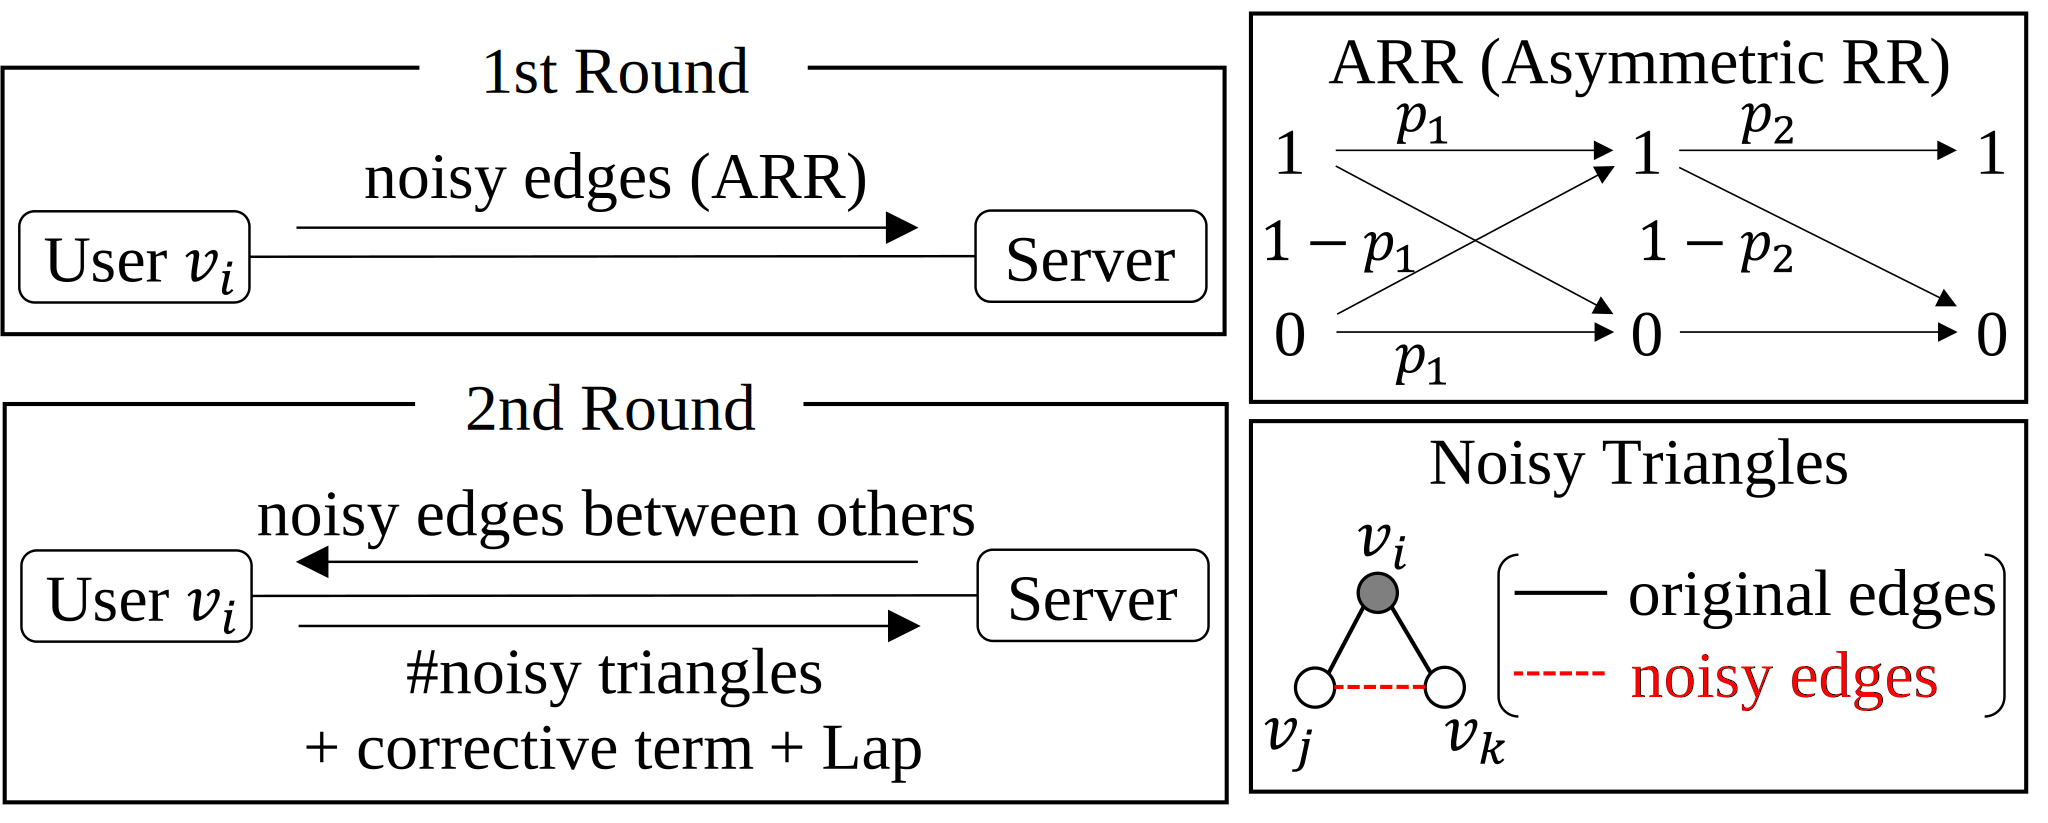
\includegraphics[width=0.99\linewidth]{fig/algorithm_overview.pdf}
  
  \caption[Overview of communication-efficient triangle counting algorithms.]
	{Overview of our communication-efficient triangle counting algorithms
  ($p_1 =\frac{e^{\epsilon}}{e^{\epsilon}+1}$,
  %$p_1 \in [\frac{1}{2},1]$,
  $p_2 \in [0,1]$).}
  %($\mu \in [0,1]$, $\rho = e^{-\epsilon_1}$).}
  %At the first round, each user obfuscates her edge by ARR ($\mu \in [0,1]$, $\rho \in e^{-\epsilon_1}$) to provide $\epsilon_1$-edge LDP.
  \label{chap2-fig:alg_overview}
\end{figure}

% \smallskip
% \noindent{\textbf{Our Two-Rounds Algorithms.}}~~
\smallskip
\noindent{\textbf{Algorithm Overview.}}~~Figure~\ref{chap2-fig:alg_overview} shows the overview of our proposed algorithms.
% all of which are run in two rounds.
% Below we explain the overview of our algorithms\footnote{For ease of explanation, we explain algorithms that use all elements in $\bmA$ in Section~\ref{chap2-sub:algorithms_overview}.
% In Section~\ref{chap2-sub:three_algorithms}, we propose algorithms that use only the lower triangular part of $\bmA$ to avoid the doubling issue, as described in Section~\ref{chap2-sub:LDP}.}.

At the first round, each user $v_i$ obfuscates
% $i-1$ bits for smaller user IDs in her neighbor list $\bma_i$ (i.e., lower triangular part of $\bmA$)
% each bit of her neighbor list $\bma_i$
% (for users with smaller user IDs)
bits for smaller user IDs in her neighbor list $\bma_i$
% (i.e., lower triangular part of $\bmA$)
by an LDP mechanism which we call the \textit{ARR (Asymmetric Randomized Response)} 
and sends the obfuscated bits to a server. 
% (note that we use only the lower triangular part of $\bmA$ to avoid the doubling issue, as described in Section~\ref{chap2-sub:LDP}).
The ARR is a combination of Warner's RR and edge sampling; i.e.,
we apply Warner's RR that outputs 1 or 0 as it is with probability
% $p_1\in[\frac{1}{2},1]$
$p_1$ ($=\frac{e^{\epsilon}}{e^{\epsilon}+1}$)
and then sample each 1 with probability $p_2\in[0,1]$.
%
% Given 1 (resp.~0) as input, the ARR outputs 1 with probability $\mu$ (resp.~$\mu\rho$), where $\mu \in [0,1]$, $\rho = e^{-\epsilon_1}$, and $\epsilon_1 \in \nnreals$.
% We can view this mechanism as a combination of Warner's RR~\cite{Warner_JASA65} and edge sampling; i.e., we apply Warner's RR that
% outputs 1 or 0 as it is with probability $p_1=\frac{e^{\epsilon_1}}{e^{\epsilon_1}+1}$
% and then sample each 1 with probability $p_2\in[0,1]$, where $\mu=p_1 p_2$.
% In fact, the ARR with $\mu = p_1$ (i.e., $p_2=1$) is equivalent to Warner's RR.
Unlike Warner's RR, the ARR is asymmetric in that the flip probability in the whole process is different
depending on the input value.
As with Warner's RR, the ARR provides edge LDP.
% Since Warner's RR provides
% $\epsilon_1$-
% edge LDP (as described in Section~\ref{chap2-sub:LDP}) and
% the sampling is a post-processing process (and
% DP is immune to post-processing~\cite{DP}, the ARR also provides
% $\epsilon_1$-
% edge LDP.
We can also significantly reduce the number of 1s (hence the communication cost) by setting
% the sampling probability
$p_2$ small.
% $\mu$ much smaller than $p_1$.
% Let $E' \subseteq V \times V$ be a set of noisy edges sent by users.

At the second round, the server calculates a message $M_i$ for user $v_i$ consisting of some or all noisy edges between others. 
We propose three strategies for calculating $M_i$. 
% and
% each user
User $v_i$ downloads $M_i$ from the server.
% a message $M_i$ from the server consisting of some or all
% of $E'$.
% noisy edges between others.
Then, since user $v_i$ knows her edges, $v_i$ can count \textit{noisy triangles} ($v_i$, $v_j$, $v_k$) such that $j<k<i$ and only one edge ($v_j$, $v_k$) is noisy, as shown in Figure~\ref{chap2-fig:alg_overview}. 
% $(v_i,v_j) \in E$, $(v_i,v_k) \in E$,
% $(v_j,v_k) \in E'$, and $j<k<i$;
% i.e., only one edge is noisy
The condition $j<k<i$ is imposed to use only the lower triangular part of $\bmA$, i.e., 
to avoid the doubling issue in Section~\ref{chap2-sub:LDP}. 
% Then $v_i$ adds some post-processing (to enable the server to obtain an unbiased estimate of $f_\triangle(G)$) and the Laplacian noise (to provide $\epsilon_2$-edge LDP for $\epsilon_2 \in \nnreals$) to the noisy triangle count, and sends it to a server.
User $v_i$ adds %some post-processing
a corrective term
%(to enable the server to obtain an unbiased estimate of $f_\triangle(G)$) 
and the Laplacian noise
% (to provide edge LDP)
to the noisy triangle count 
and sends it to a server.
The corrective term is added to enable the server to obtain an unbiased estimate of $f_\triangle(G)$. 
The Laplacian noise provides
% $\epsilon_2$-
edge LDP.
% , where $\epsilon_2 \in \nnreals$.
% From this,
Finally,
the server calculates an unbiased estimate of $f_\triangle(G)$
from the noisy data sent by users.
By composition (Proposition~\ref{chap2-prop:seq_comp_edge_LDP}),
% the compositionality of DP~\cite{DP},
our algorithms provide
% ($\epsilon_1 + \epsilon_2$)-
edge LDP in total.

\smallskip
\noindent{\textbf{Remark.}}~~Note that it is also possible for the server to calculate an unbiased estimate of $f_\triangle(G)$ at the first round.
However, this results in a
prohibitively
% very
large estimation error
% for a large graph
% for two reasons.
because
% First,
all edges sent by users are noisy; i.e., three edges are noisy in any triangle.
% all three edges are noisy in any triangle at the first round (whereas only one edge is noisy in our algorithms),
% Second, the noisy graph is dense, and consequently the time complexity of counting noisy triangles is $O(n^3)$. Thus, some approximation (such as edge sampling) is necessary to efficiently compute the estimate of $f_\triangle(G)$.
In contrast, only one edge is noisy in each noisy triangle at the second round because each user $v_i$ knows two original edges
% $(v_i,v_j) \in E$ and $(v_i,v_k) \in E$
connected to $v_i$.
Consequently, we can obtain an unbiased estimate with a much smaller variance.
See Appendix~\ref{chap2-sec:one-round} for a detailed comparison.
% In Appendix~\ref{chap2-sec:one-round}, we show that
% our two-rounds algorithms significantly outperform the existing one-round triangle algorithms.
% ~\cite{Imola_USENIX21,Ye_TKDE21}.
% (with sampling).
% the estimation error is significantly reduced by introducing an additional round.

% \subsection{Three Algorithms}
\subsection{Algorithms}
\label{chap2-sub:three_algorithms}

\smallskip
\noindent{\textbf{ARR.}}~~First, we formally define the ARR.
% We begin with a formal definition of the ARR.
% Below we describe our algorithms in detail.
The ARR has two parameters: $\epsilon \in \nnreals$ and $\mu \in [0,\frac{e^{\epsilon}}{e^{\epsilon} + 1}]$.
The parameter $\epsilon$ is the privacy budget, and $\mu$ controls the communication cost.

Let
% $\calR_{ARR}$
$ARR_{\epsilon,\mu}$ be the ARR with parameters $\epsilon$ and $\mu$. It takes $0/1$ as input and outputs $0/1$ with the following probability:
\begin{align}
    \Pr[ARR_{\epsilon,\mu}(1) = b] &= \begin{cases}\mu & (b=1) \\ 1-\mu & (b=0)\end{cases} \label{chap2-eq:ARR_1}\\
    \Pr[ARR_{\epsilon,\mu}(0) = b] &= \begin{cases}\mu\rho & (b=1) \\ 1-\mu \rho & (b=0), \end{cases} \label{chap2-eq:ARR_0}
\end{align}
where $\rho = e^{-\epsilon}$.
By Figure~\ref{chap2-fig:alg_overview},
we can view this randomizer as a combination of Warner's RR~\cite{Warner_JASA65}
% with $p_1=\frac{e^{\epsilon}}{e^{\epsilon}+1}$
and edge sampling, where $\mu=p_1 p_2$.
In fact, the ARR with $\mu = p_1 =\frac{e^{\epsilon}}{e^{\epsilon}+1}$ (i.e., $p_2=1$) is equivalent to Warner's RR.

Each user $v_i$ applies the ARR to bits for smaller user IDs in her neighbor list $\bma_i$; i.e., $\calR_i(\bma_i) = (ARR_{\epsilon,\mu}(a_{i,1}), \ldots, \allowbreak ARR_{\epsilon,\mu}(a_{i,i-1}))$.
% Note that we use only the lower triangular part of $\bmA$ to avoid the doubling issue described in Section~\ref{chap2-sub:LDP}.
Then $v_i$ sends $\calR_i(\bma_i)$ to the server.
% Applying Warner's RR to each bit of $\bma_i$ provides $\epsilon$-edge LDP (as described in Section~\ref{chap2-sub:LDP}).
Since applying Warner's RR to $\bma_i$ provides $\epsilon$-edge LDP (as described in Section~\ref{chap2-sub:LDP}) and the sampling is a post-processing process, applying the ARR to $\bma_i$ also provides $\epsilon$-edge LDP by the immunity to post-processing~\cite{DP}.

Let $E' \subseteq V \times V$ be a set of noisy edges sent by users.

\smallskip
\noindent{\textbf{Which Noisy Edges to Download?}}~~Now, the main question
tackled in this paper is: \textit{Which noisy edges should each user $v_i$
download at the second round?}
Note that
% user $v_i$ cannot leak her original edges to the server.
% For example,
user $v_i$
% cannot
is not allowed to
download only a set of noisy edges that form noisy triangles
(i.e., $\{(v_j,v_k) \in E' | (v_i,v_j) \in E, (v_i,v_k) \in E$\}),
% a set of noisy edges $\{(v_j,v_k) \in E' | (v_i,v_j) \in E, (v_i,v_k) \in E$\} (i.e., only noisy edges that form noisy triangles),
because it tells the server
% the fact that $v_j$ and $v_k$ are friends with $v_i$.
who are friends with $v_i$.
In other words, user $v_i$ cannot leak her original edges to the server when she
downloads noisy edges; the server must choose which part of $E'$ to include in
the message $M_i$ it sends her.

Thus, a natural solution would be to download \textit{all noisy edges between others}
% (except for the ones connected to $v_i$).
(with smaller user IDs); i.e.,
% \begin{align}
% M_i =\{(v_j, v_k) \in E' | j<k<i\}. \label{chap2-eq:M_i_I}
% \end{align}
$M_i =\{(v_j, v_k) \in E' | j<k<i\}$.
% as shown in Figure~\ref{chap2-fig:noisy_edge_DL}.
We denote our algorithm with this full download strategy by \AlgOne{}.
The (inefficient) two-rounds algorithm in~\cite{Imola_USENIX21} is a special case of \AlgOne{}
without sampling ($\mu = p_1$).
% when $\mu = p_1$ (i.e., when we
% use Warner's RR and
% do not sample edges).
In other words, \AlgOne{} is a generalization of the two-rounds algorithm in~\cite{Imola_USENIX21} using the ARR.
% $(v_j,v_k) \in E'$ such that $(v_i,v_j) \in E$, $(v_i,v_k) \in E$
% The expected download size in \AlgOne{} is $O(\mu n^2)$.

% Since users have already sent noisy edges at the first round, user $v_i$ can use noisy edges connected to $v_i$ when downloading noisy edges.
% For example,

In this paper,
we show that we can do much better
% we achieve much higher utility
than \AlgOne{}.
Specifically, we prove in Section~\ref{chap2-sub:algorithms_theoretical_analysis} that \AlgOne{} results in a high estimation error when the number of 4-cycles (cycles of length 4) in $G$ is large.
Intuitively, this can be explained as follows.
Suppose that $v_i$, $v_j$, $v_{i'}$, and $v_k$
($j<k<i$, $j<k<i'$)
form a 4-cycle. 
% $v_i-v_j-v_{i'}-v_k-v_i$.
% (denoted by $v_i$-$v_j$-$v_{i'}$-$v_k$).
% , as shown in the left panel of Figure~\ref{chap2-fig:four-cycle}.
There is no triangle in this graph.
However, if there is a noisy edge between $v_j$ and $v_k$, then two (incorrect) noisy triangles appear: ($v_i$, $v_j$, $v_k$) counted by $v_i$ and ($v_{i'}$, $v_j$, $v_k$) counted by $v_{i'}$.
More generally, let $E_{ijk}$ (resp.~$E_{i'jk}$) $\in \{0,1\}$ be a random variable that takes $1$ if ($v_i$, $v_j$, $v_k$) (resp.~($v_{i'}$, $v_j$, $v_k$)) forms a noisy triangle and $0$ otherwise.
Then, the covariance $\cov(E_{ijk},E_{i'jk})$ between $E_{ijk}$ and $E_{i'jk}$ is large because the presence/absence of a single noisy edge ($v_j$, $v_k$) affects the two noisy triangles.

To address this issue, we introduce a
% \textit{trick}
trick 
% trick, which we call the ``$4$-cycle trick'',
that makes the two noisy triangles \textit{less correlated with each other}.
We call this the \textit{4-cycle trick}.
% Since users have already sent noisy edges at the first round,
% user $v_i$ can use noisy edges connected to $v_i$ when downloading noisy edges.
Specifically,
% we propose two algorithms: \AlgTwo{} and \AlgThree{}.
we propose two algorithms in which
% user $v_i$ uses noisy edges connected to $v_i$ when downloading noisy edges.
the server uses noisy edges connected to $v_i$ when it calculates a message $M_i$ for $v_i$.
In the first algorithm,
% user $v_i$ downloads
the server selects
noisy edges $(v_j, v_k)$ such that
one noisy edge is connected from $v_k$ to $v_i$;
% there is a noisy edge between $v_i$ and $v_k$;
i.e.,
$M_i = \{(v_j, v_k) \in E' | (v_i, v_k) \in E', j<k<i\}$.
% \begin{align}
% M_i = \{(v_j, v_k) \in E' | (v_i, v_k) \in E', j<k<i\}. \label{chap2-eq:M_i_II}
% \end{align}
We call this algorithm \AlgTwo{}, as one noisy edge is connected to $v_i$.
In the second algorithm,
% user $v_i$ downloads
the server selects
noisy edges $(v_j, v_k)$ such that
two noisy edges are connected from these nodes to $v_i$; i.e.,
$M_i = \{(v_j, v_k) \in E' | (v_i, v_j) \in E', (v_i, v_k) \in E', j<k<i\}$.
% \begin{align}
% \hspace{-2mm} M_i \hspace{-0.5mm} = \hspace{-0.5mm}  \{(v_j, v_k) \in E' | (v_i, v_j) \in E', (v_i, v_k) \in E', j<k<i\}. \label{chap2-eq:M_i_III}
% \end{align}
We call this algorithm \AlgThree{}, as two noisy edges are connected to $v_i$.
Note that user $v_i$ does not leak her original edges to the server at the time of download in these algorithms, because
% $v_i$ uses only noisy edges the server has.
the server uses only noisy edges $E'$ sent by users to calculate $M_i$.

Figure~\ref{chap2-fig:noisy_edge_DL} shows our three algorithms.
% Let $\mu_F, \mu_O, \mu_T \in \nnreals$ be values of $\mu$ in the ARR used for \AlgOne{}, \AlgTwo{}, and \AlgThree{}, respectively.
% Then the
The download cost $\CostDL{}$ in (\ref{chap2-eq:cost_DL}) is
$O(\mu n^2 \log n)$, $O(\mu^2 n^2 \log n)$, and $O(\mu^3 n^2 \log n)$,
% $O(\mu_F n^2 \log n)$, $O(\mu_O^2 n^2 \log n)$, and $O(\mu_T^3 n^2 \log n)$,
respectively, when we regard $\epsilon$ as a constant.
In our experiments, we set
the parameter $\mu$ in the ARR so that
% $\mu$ in \AlgOne{}, $\mu^2$ in \AlgTwo{}, and $\mu^3$ in \AlgThree{} are equal
$\mu$ in \AlgOne{} is equal to $\mu^2$ in \AlgTwo{} and also equal to $\mu^3$ in \AlgThree{};
e.g., $\mu=10^{-6}$, $10^{-3}$, and $10^{-2}$ in \AlgOne{}, \AlgTwo{}, and \AlgThree{}, respectively.
% $\mu_F$, $\mu_O$, and $\mu_T$ to $\mu_F = \mu_O^2 = \mu_T^3$ (e.g., $\mu_F=10^{-6}$, $\mu_O=10^{-3}$, $\mu_T=10^{-2}$)
% so that
% the expected download size
Then
the download cost
is the same between the three algorithms.

\begin{figure}[t]
  \centering
  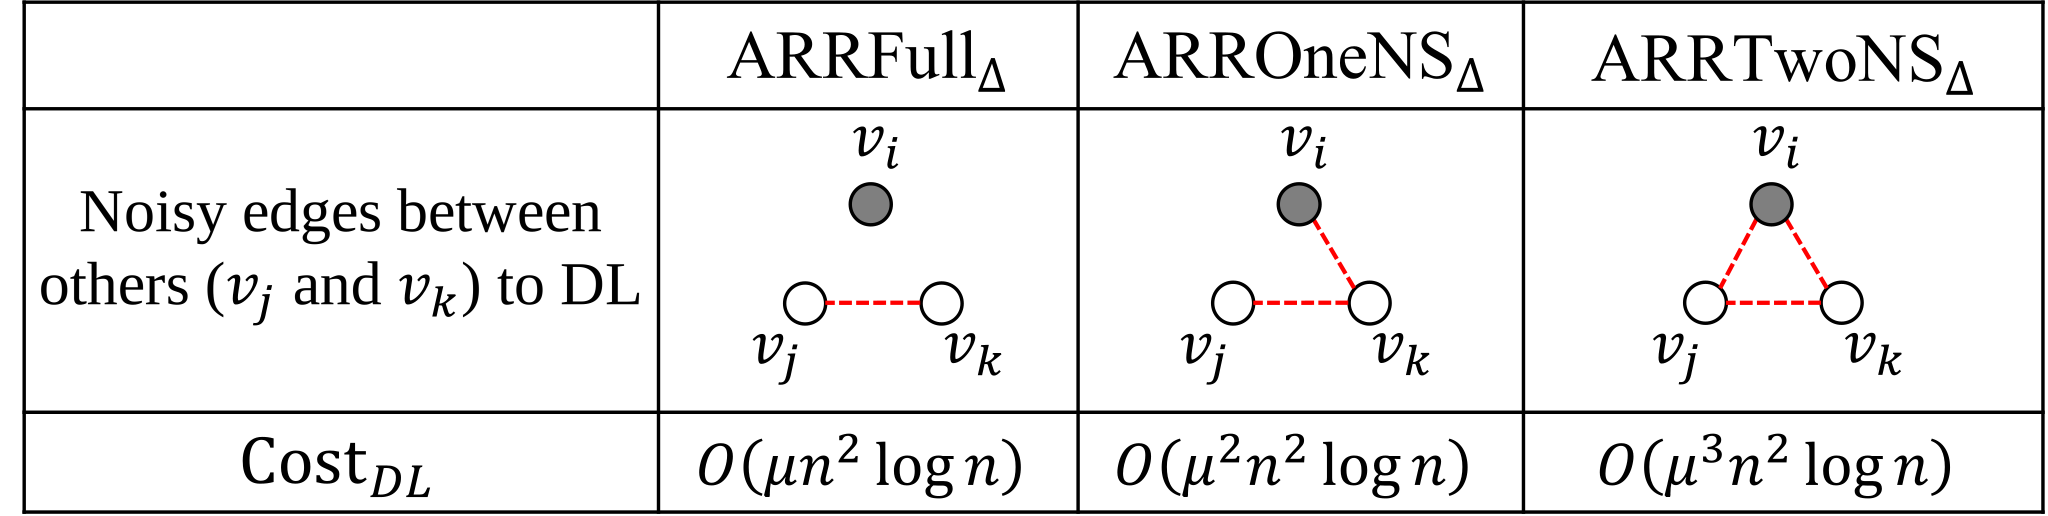
\includegraphics[width=0.99\linewidth]{fig/three_algorithms.pdf}
  
  \caption[Noisy edges to download in our three algorithms.]{Noisy edges to download
  in our three algorithms.}
  %$\mu_F$, $\mu_O$, and $\mu_T$ are values of $\mu$ in the ARR used for \AlgOne{}, \AlgTwo{}, and \AlgThree{}, respectively.}
  \label{chap2-fig:noisy_edge_DL}
% \end{figure}
\vspace{4mm}
% \begin{figure}[t]
  \centering
  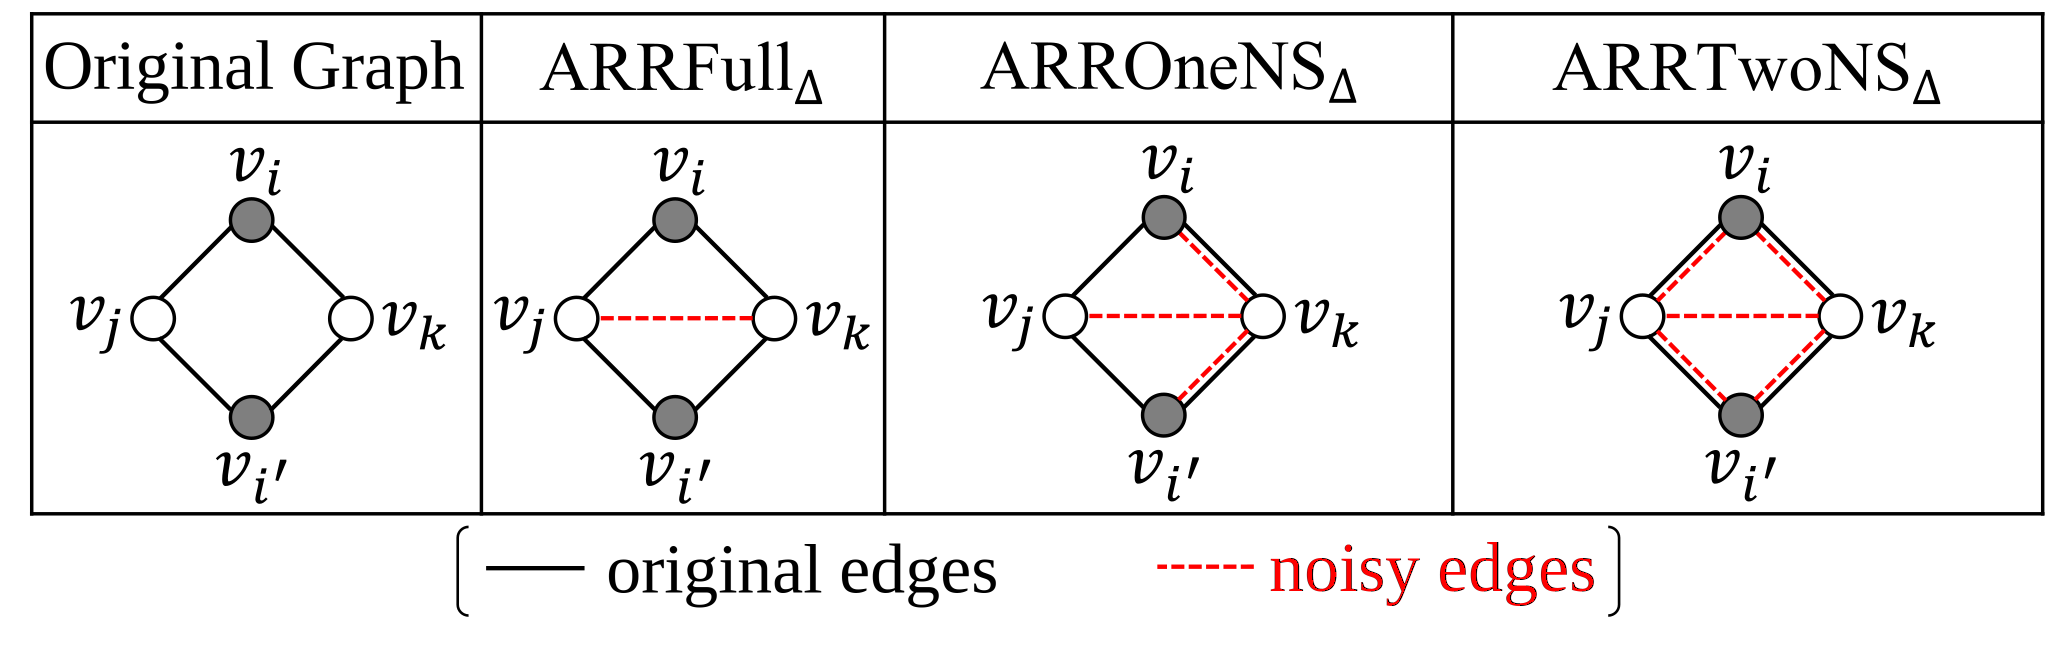
\includegraphics[width=0.95\linewidth]{fig/four_cycle.pdf}
  
  \caption[4-cycle trick]{4-cycle trick.
  % 4-cycle issue.
  \AlgOne{} counts two (incorrect) noisy triangles when one noisy edge appears.
  \AlgTwo{} and \AlgThree{} avoid this by increasing independent noise.}
  \label{chap2-fig:four-cycle}
\end{figure}

% Figure\ref{chap2-fig:four-cycle} shows why and how \AlgTwo{} and \AlgThree{} address the 4-cycle issue.
Figure~\ref{chap2-fig:four-cycle} shows our $4$-cycle trick.
\AlgOne{} counts two (incorrect) noisy triangles when a noisy edge ($v_j$, $v_k$) appears.
% there is a noisy edge ($v_j$, $v_k$).
In contrast,
% the two noisy triangles are counted
\AlgTwo{} (resp.~\AlgThree{}) counts both the two noisy triangles
% this bad event happens
only when three (resp.~five) independent noisy edges appear,
% in \AlgTwo{} (resp.~\AlgThree{}),
as shown in Figure~\ref{chap2-fig:four-cycle}.
% Since these noisy edges are independent,
Thus, this bad event happens with a much smaller probability.
For example,
% when $\mu_F=10^{-6}$, $\mu_O=10^{-3}$, and $\mu_T=10^{-2}$,
% \AlgOne{}, \AlgTwo{}, and \AlgThree{} count both the two noisy triangles with probability $10^{-6}$, $10^{-9}$, and $10^{-10}$, respectively.
\AlgOne{} ($\mu=10^{-6}$),
\AlgTwo{} ($\mu=10^{-3}$), and
\AlgThree{} ($\mu=10^{-2}$)
count both the two noisy triangles with probability $10^{-6}$, $10^{-9}$, and $10^{-10}$, respectively.
The covariance $\cov(E_{ijk},E_{i'jk})$ of \AlgTwo{} and \AlgThree{} is also much smaller than that of \AlgOne{}.
% \AlgTwo{} and \AlgThree{} also achieve much smaller covariance $\cov(E_{ijk},E_{i'jk})$ than \AlgOne{}.


In our experiments, we show that \AlgTwo{} and \AlgThree{} significantly outperforms \AlgOne{}
% in two real graph datasets with a large number of 4-cycles.
for a large-scale graph or dense graph, in both of which
% when
the number of 4-cycles in $G$ 
% can be very 
is 
large.
% \ji{Are there other scenarios where the performance is better?}
% \commentT{I think the number of 4-cycles can be large when a graph is (i) large or (ii) dense (in particular, (i) is important). I clarified this.}

\smallskip
\noindent{\textbf{\AlgTwo{} vs. \AlgThree{}.}}~~One
% The number of independent noisy edges in a 4-cycle is three and five in \AlgTwo{} and \AlgThree{}, respectively, as shown in Figure\ref{chap2-fig:four-cycle}.
% Thus
might expect that \AlgThree{} outperforms \AlgTwo{} because \AlgThree{} addresses the 4-cycle issue more aggressively; i.e.,
% \AlgThree{} has the largest number of independent noisy edges in a 4-cycle,
the number of independent noisy edges in a 4-cycle is larger in \AlgThree{},
as shown in Figure \ref{chap2-fig:four-cycle}.
However,
% \AlgThree{} suffers from a large global sensitivity of the Laplacian noise at the second round.
\AlgTwo{} can reduce the global sensitivity of the Laplacian noise
at the second round
more effectively than \AlgThree{}, as explained in Section~\ref{chap2-sec:double_clip}.
% in detail.
Consequently, \AlgTwo{}, which is the most tricky algorithm, achieves the smallest estimation error in our experiments.
See Sections~\ref{chap2-sec:double_clip} and \ref{chap2-sec:experiments} for details of the global sensitivity and experiments, respectively.

\smallskip
\noindent{\textbf{Three Algorithms.}}~~Below we explain the details of our three algorithms.
For ease of explanation, we assume that the maximum degree $d_{max}$ is public in Section~\ref{chap2-sub:three_algorithms}\footnote{For example, $d_{max}$ is public in Facebook: $d_{max} = 5000$~\cite{Facebook_Limit}.
If the server does not have prior knowledge about $d_{max}$, she can privately estimate $d_{max}$ and use graph projection to guarantee that each user's degree never exceeds the private estimate of $d_{max}$~\cite{Imola_USENIX21}.
In any case, the assumption in Section~\ref{chap2-sub:three_algorithms} does not undermine our algorithms, because our entire algorithms with double clipping in Section~\ref{chap2-sec:double_clip} does \textit{not} assume that $d_{max}$ is public.}.
Note, however, that
% we propose a technique to significantly reduce the global sensitivity
our double clipping (which is proposed to significantly reduce the global sensitivity) in Section~\ref{chap2-sec:double_clip} does \textit{not} assume that $d_{max}$ is public.
Consequently, our entire algorithms 
% (i.e., \AlgOne, \AlgTwo, \AlgThree with double clipping)
% three triangle counting algorithms (\AlgOne, \AlgTwo, \AlgThree) with our double clipping
do \textit{not} require the assumption that $d_{max}$ is public.

\setlength{\algomargin}{5mm}
\begin{algorithm}[t]
  \SetAlgoLined
  \KwData{Graph $G \in \calG$ represented as neighbor lists $\bma_1, \ldots, \bma_n
    \in \{0,1\}^n$, privacy budgets
  $\epsilon_1,\epsilon_2 \in \nnreals$, $d_{max} \in \nnints$,
  $\mu \in [0,\frac{e^{\epsilon_1}}{e^{\epsilon_1} + 1}]$.
  %$\mu^*$.
  }
  \KwResult{Private estimate $\hf_\triangle(G)$ of $f_\triangle(G)$.}
%   $p_1 \leftarrow \frac{1}{e^{\epsilon_1}}$\;
  [s] $\rho \leftarrow e^{-\epsilon_1}$\;
  [$v_i$, s] $\mu^* \leftarrow \mu$, $\mu^2$, and $\mu^3$ in F, O, and T, respectively\;
  \tcc{First round.}
  \For{$i=1$ \KwTo $n$}{
    [$v_i$] $\bmr_i \leftarrow (ARR_{\epsilon_1,\mu}(a_{i,1}), \ldots,
    ARR_{\epsilon_1,\mu}(a_{i,i-1}))$\;
    [$v_i$] Upload $\bmr_i = (r_{i,1}, \ldots, r_{i,i-1})$ to the server\;
  }
%   $E' = \{(v_i, v_j) : i > j, r_{i,j} = 1\} \cup \{(v_j, v_i) : i > j, r_{i,j} =
%   1\}$\;
  [s] $E' = \{(v_j, v_k) :r_{k,j} = 1, j < k\}$\;
  \tcc{Second round.}
  \For{$i=1$ \KwTo $n$}{
    [s] Compute
    $M_i$ by (\ref{chap2-eq:M_i_I}), (\ref{chap2-eq:M_i_II}), and (\ref{chap2-eq:M_i_III}) in F, O, and T, respectively\;
    %$M_i = \{(v_j,v_k) \in E': j < k < i\}$\;
    %$M_i = \{(v_j,v_k) \in E': (v_i,v_k) \in E', j < k < i\}$\;
    %$M_i = \{(v_j,v_k) \in E': (v_i,v_k), (v_j,v_k) \in E', j < k < i\}$\;
    [$v_i$] Download $M_i$ from the server\;
    [$v_i$] $t_i \leftarrow |\{(v_i,v_j,v_k) :
    a_{i,j} = a_{i,k} = 1, (v_j,v_k) \in M_i, j<k<i \}|$\;
    [$v_i$] $s_i \leftarrow |\{(v_i,v_j,v_k) :
    a_{i,j} = a_{i,k} = 1, j<k<i\}|$\;
    [$v_i$] $w_i \leftarrow t_i - \mu^* \rho s_i$\;
    [$v_i$] $\hw_i \leftarrow w_i + \Lap(\frac{d_{max}}{\epsilon_2})$\;
    [$v_i$] Upload $\hw_i$ to the server\;
  }
  [s] $\hf_\triangle(G) \leftarrow \frac{1}{\mu^*(1-\rho)}\sum_{i=1}^n \hw_i$\;
  \KwRet{$\hf_\triangle(G)$}
  \caption[Definition of our three algorithms.]{Our three algorithms.
  ``F'', ``O'', ``T'' are shorthands for
  %$\mu^*=\mu_F$, $\mu_O^2$, and $\mu_T^3$ in
  \AlgOne{}, \AlgTwo{}, and \AlgThree{}, respectively.
  [$v_i$] and [s] represent that the process is run by $v_i$ and the server, respectively.
  }\label{chap2-alg:unify}
\end{algorithm}

% As explained above,
Recall that the server calculates a message $M_i$ for $v_i$ as:
\begin{align}
\hspace{-1mm} M_i \hspace{-0.5mm} &= \hspace{-0.5mm} \{(v_j, v_k) \in E' | j<k<i\} \label{chap2-eq:M_i_I}\\
\hspace{-1mm} M_i \hspace{-0.5mm} &= \hspace{-0.5mm} \{(v_j, v_k) \in E' | (v_i, v_k) \in E', j<k<i\} \label{chap2-eq:M_i_II}\\
\hspace{-1mm} M_i \hspace{-0.5mm} &= \hspace{-0.5mm}  \{(v_j, v_k) \in E' | (v_i, v_j) \in E', (v_i, v_k) \in E', j<k<i\} \label{chap2-eq:M_i_III}
\end{align}
in \AlgOne{}, \AlgTwo{}, \AlgThree{}, respectively.

%Using these equations,
% our three algorithms can be unified in Algorithm~\ref{chap2-alg:unify}.
Algorithm~\ref{chap2-alg:unify} shows our three algorithms.
These algorithms are processed differently in lines 2 and 9; ``F'', ``O'', ``T'' are shorthands for \AlgOne{}, \AlgTwo{}, and \AlgThree{}, respectively.
% It uses two rounds of private computation, and
% in both rounds each user $v_i$ applies a local randomizer to her neighbor list $\bma_i$.
The privacy budgets for the first and second
rounds are $\epsilon_1, \epsilon_2 \in \nnreals$, respectively.

The first round appears in lines 3-7 of Algorithm~\ref{chap2-alg:unify}.
In this round, each user applies
$ARR_{\epsilon_1, \mu}$
% the ARR
defined by (\ref{chap2-eq:ARR_1}) and (\ref{chap2-eq:ARR_0}) to bits $a_{i,1}, \ldots, a_{i,i-1}$ for smaller user IDs in her neighbor list $\bma_i$, i.e., lower triangular part of $\bmA$.
% explained in the beginning of
% Section~\ref{chap2-sub:three_algorithms}.
Let $\bmr_i = (r_{i,1}, \ldots, r_{i,i-1}) \in \{0,1\}^{i-1}$ be the obfuscated bits of $v_i$.
User $v_i$ uploads $\bmr_i$ to the server.
Then the server combines the noisy edges together, forming $E' = \{(v_j, v_k) : r_{k,j} = 1, j < k\}$.

The second round appears in lines 8-17 of Algorithm~\ref{chap2-alg:unify}.
In this round, the server computes a message $M_i$
by (\ref{chap2-eq:M_i_I}), (\ref{chap2-eq:M_i_II}), or (\ref{chap2-eq:M_i_III}),
% depending on the algorithm,
and user $v_i$ downloads it.
% As explained above, \AlgOne{}, \AlgTwo{}, and \AlgThree{} computes $M_i$ by (\ref{chap2-eq:M_i_I}), (\ref{chap2-eq:M_i_II}), and  (\ref{chap2-eq:M_i_III}), respectively.
Then user $v_i$ calculates the number $t_i \in \nnints$ of noisy triangles ($v_i$, $v_j$, $v_k$) such that
% $j<k<i$ and
only one edge ($v_j$, $v_k$) is noisy, as shown in Figure~\ref{chap2-fig:alg_overview}.
% involving two edges in user $v_i$'s neighbor list and one noisy edge in $E'$ (as shown in Figure~\ref{chap2-fig:alg_overview}).
% We also emphasize that the condition $j<k<i$ is imposed to use only the lower triangular part of $\bmA$.
% (and avoid the doubling issue).
User $v_i$ also calculate a corrective term $s_i \in \nnints$.
The corrective term $s_i$ is the number of
possible triangles involving $v_i$ 
% that can be formed from edges in $v_i$'s neighbor list,
and is computed to obtain an unbiased estimate of $f_\triangle(G)$.
% unbias the triangle count.
User $v_i$ calculates $w_i = t_i - \mu^* \rho s_i$, where $\rho = e^{-\epsilon_1}$ and
% $\mu^* = \mu_F$, $\mu_O^2$, and $\mu_T^3$
$\mu^* = \mu$, $\mu^2$, and $\mu^3$
in ``F'', ``O'', and ``T'', respectively.
% \AlgOne{}, \AlgTwo{}, and \AlgThree{}, respectively.
Then $v_i$ adds the Laplacian noise $\Lap(\frac{d_{max}}{\epsilon_2})$ to $w_i$ to provide $\epsilon_2$-edge LDP and sends the noisy value $\hw_i$ ($= w_i + \Lap(\frac{d_{max}}{\epsilon_2})$) to the server. 
Note that adding one edge increases both $t_i$ and $s_i$ 
% results in the increase of the triangle count 
by at most $d_{max}$. 
Thus, the global sensitivity of $w_i$ is at most $d_{max}$. 
Finally, the server calculates an estimate of $f_\triangle(G)$ as: $\hf_\triangle(G) = \frac{1}{\mu^*(1-\rho)}\sum_{i=1}^n \hw_i$.
As we prove later, $\hf_\triangle(G)$ is an unbiased estimate of $f_\triangle(G)$.

% \smallskip
% \noindent{\textbf{\AlgOne.}}

% Our first algorithm, \AlgOne, appears in Algorithm~\ref{chap2-alg:one}. It uses two
% rounds of private computation, and in both rounds each user applies a local
% randomizer to his data.
% The privacy budgets for the two
% rounds are $\epsilon_1, \epsilon_2$.

% The first round appears in Lines 3-4 of Algorithm~\ref{chap2-alg:one}. This round
% collects the noisy edges from the users.
% The noisy edges are produced
% using the asymmetric randomized response mechanism, which we denote
% $ARR_{\epsilon, \mu}$. Recall that a bit $a_{i,j}$ of $\bma_i$ takes value $1$
% if and only if user $v_i$ includes user $v_j$ in his neighbor list. ARR is
% defined by $\Pr[ARR_{\epsilon, \mu}(1) = 1] = \mu$ and $\Pr[ARR_{\epsilon,
% \mu}(0) = 1] = \mu p_1$ where $p_1 = e^{-\epsilon_1}$. User $v_i$ uploads
% $\bmr_i$, the vector of ARR mechanisms applied to $a_{i,j}$ for $j < i$. This
% means that user $v_i$ ignores users with a bigger index than $i$. By doing so,
% for every possible undirected edge $(v_i, v_j)$, exactly one of $v_i, v_j$ will
% upload the
% edge using ARR. This prevents releasing the edge twice, and allows us to prove
% that our mechanism satisfies relationship DP without the doubling factor in
% $\epsilon$ (see Proposition~\ref{chap2-prop:edge_LDP_entire_edge_LDP}).
% Given the collection of ARR queries to the users, the server concludes the first
% round by combining the noisy edges together and unordering them, forming $E'$.

% The second round appears in Lines 8-13 of Algorithm~\ref{chap2-alg:one}.
% In this round, each user $v_i$ computes an unbiased estimator $w_i$ for
% the number of triangles involving $v_i$ for which the maximum index of the
% triangle is $i$. It is easy to see that the sum of the $w_i$ estimates the total
% number of triangles. The user does this by
% downloading the message $M = E'$ from the server
% and computing a noisy triangle count $t_i$ and a corrective term $s_i$. The count
% $t_i$ is the number of triangles involving two edges in user $v_i$'s neighbor
% list and one noisy edge in $E'$. The corrective term $s_i$ is the number of
% possible triangles that can be formed from edges in user $v_i$'s neighbor list,
% and is computed to unbias the triangle count. We emphasize that user $v_i$
% only considers the part of his neighbor list involving users of a lower index
% than $i$ for all calculations, including this. The unbiased estimator is
% given by $w_i = t_i - \mu_F p_1 s_i$---because it depends on the private data
% $\bma_i$, the user adds Laplacian noise of width $\frac{d_{max}}{\epsilon_2}$ to
% $w_i$ that the computation may satisfy $\epsilon_2$ edge LDP. He then uploads
% the noisy value $\hw_i$, and the server computes the final triangle estimate.

% \begin{algorithm}
%   \SetAlgoLined
%   \KwData{Graph $G$ represented as neighbor lists $\bma_1, \ldots, \bma_n
%     \in \{0,1\}^n$, two privacy budgets
%   $\epsilon_1,\epsilon_2 > 0$, $d_{max} \in \nnints$, sampling parameter
%   $\mu_F$.}
%   \KwResult{Private estimate of $f_\triangle(G)$.}
%   $p_1 \leftarrow \frac{1}{e^{\epsilon_1}}$\;
%   \tcc{First round.}
%   \For{$i=1$ \KwTo $n$}{
%     $\bmr_i \leftarrow (ARR_{\epsilon_1,\mu_F}(a_{i,1}), \ldots,
%     ARR_{\epsilon_1,\mu_F}(a_{i,i-1}))$\;
%     Upload $\bmr_i$ to server\;
%   }
%   $E' = \{(v_j, v_i) : i > j, r_{i,j} = 1\}$\;
%   \tcc{Second round.}
%   \For{$i=1$ \KwTo $n$}{
%     Server lets $M_i = E'$.
%     Download $M_i$ from server\;
%     $t_i \leftarrow |\{(v_i,v_j,v_k) :
%     j<k<i, a_{i,j} = a_{i,k} = 1, (k,j) \in M \}|$\;
%     $s_i \leftarrow |\{(v_i,v_j,v_k) :
%     j<k<i, a_{i,j} = a_{i,k} = 1\}|$\;
%     $w_i \leftarrow t_i - \mu_F p_1 s_i$\;
%     $\hw_i \leftarrow w_i + \Lap(\frac{d_{max}}{\epsilon_2})$\;
%     Upload $\hw_i$ to server\;
%   }
%   \KwRet{$\frac{1}{\mu_F(1-p_1)}\sum_{i=1}^n \hw_i$}
%   \caption{\AlgOne}\label{chap2-alg:one}
% \end{algorithm}

% \smallskip
% \noindent{\textbf{\AlgTwo.}}

% Our second Algorithm, \AlgTwo, appears in Algorithm~\ref{chap2-alg:two}. Like
% \AlgOne, it uses two rounds with budgets $\epsilon_1$ and $\epsilon_2$.
% The first round is identical to \AlgOne, and for brevity, Algorithm~\ref{chap2-alg:two} does not
% include a description of the first round.
% Recall that the goal of the second round is for each user $v_i$ to compute an estimate of the
% number of triangles in which $i$ is the maximum index, which is the variable
% $\hw_i$.
% The difference between \AlgOne and
% \AlgTwo is that in the second round of \AlgTwo (Lines 2-8), a user only downloads a
% subset of edges in
% $E'$: $v_i$ downloads those edges $(v_j, v_k) \in E'$ such that $j < k < i$ and
% $v_i \text{\----} v_k \text{\----} v_j$ are connected in $E'$. The server is
% able to compute these edges since they only depend on the first round release,
% and we denote it with $M_i$. User $v_i$ then computes his estimate $w_i = t_i -
% \mu_O^2 p_1 s_i$, where $t_i$ is and $s_i$ are the same quantities as in
% \AlgOne. The final estimator $w_i = t_i - \mu_O^2
% p_1 s_i$ is an unbiased estimate of the number of triangles for which $i$ is the
% maximum index. User $v_i$ uploads $\hw_i$, given by $w_i$ plus Laplace noise, in
% order to share $w_i$ privately.

% Downloading only some of $E'$, depending on the noisy first round, actually
% produces a noisier estimator $\hw_i$ than \AlgOne. However, the communication
% cost of \AlgTwo is less, precisely because a subset of $E'$ is downloaded. It
% is straightforward to prove that in expectation, user $v_i$ downloads $\mu_F
% n^2$ edges in \AlgOne and $\mu_O^2 n^2$ edges in \AlgTwo. Thus, the two
% algorithms have comparable communication when $\mu_F = \mu_O^2$, meaning that
% $\mu_F \ll \mu_O$. Thus, \AlgOne is forced to sample edges at a much smaller
% ratio than \AlgTwo in the first round, producing a much noisier value of $E'$.
% At these two different sampling ratios, the estimator $\hw_i$ in \AlgTwo is not
% necessarily worse than the same estimator in \AlgOne

% \begin{algorithm}
%   \SetAlgoLined
%   \KwData{Graph $G$ represented as neighbor lists $\bma_1, \ldots, \bma_n
%     \in \{0,1\}^n$, two privacy budgets
%   $\epsilon_1,\epsilon_2 > 0$, $d_{max} \in \nnints$, sampling parameter
%   $\mu_O$.}
%   \KwResult{Private estimate of $f_\triangle(G)$.}
%   \tcc{Second round.}
%   \For{$i=1$ \KwTo $n$}{
%     Server computes $M_i = \{(j,k) : j < k < i, (k,i), (j,k) \in E'\}$\;
%     Download $M_i$ from server\;
%     $t_i \leftarrow |\{(v_i,v_j,v_k) :
%     j<k<i, a_{i,j} = a_{i,k} = 1, (j,k) \in M_i\}|$\;
%     $s_i \leftarrow |\{(v_i,v_j,v_k) :
%     j<k<i, a_{i,j} = a_{i,k} = 1\}|$\;
%     $w_i \leftarrow t_i - \mu_O^2 p_1 s_i$\;
%     $\hw_i \leftarrow w_i + \Lap(\frac{d_{max}}{\epsilon_2})$\;
%     Upload $\hw_i$ to server\;
%   }
%   \KwRet{$\frac{1}{\mu_O^2(1-p_1)}\sum_{i=1}^n \hw_i$}
%   \caption{\AlgTwo, second round only (first round is identical to \AlgOne with
%   sampling parameter $\mu_O$).}\label{chap2-alg:two}
% \end{algorithm}

% \smallskip
% \noindent{\textbf{\AlgThree.}}~~TBD
% \colorB{\begin{itemize}
%     \item Algorithm of \AlgThree (only the 2nd round).
% \end{itemize}}

% \begin{algorithm}
%   \SetAlgoLined
%   \KwData{Graph $G$ represented as neighbor lists $\bma_1, \ldots, \bma_n
%     \in \{0,1\}^n$, two privacy budgets
%   $\epsilon_1,\epsilon_2 > 0$, $d_{max} \in \nnints$, sampling parameter
%   $\mu_T$.}
%   \KwResult{Private estimate of $f_\triangle(G)$.}
%   \tcc{Second round.}
%   \For{$i=1$ \KwTo $n$}{
%     Server computes $M_i = \{(j,k) : j < k < i, (k,i), (j,k), (j,i) \in E'\}$\;
%     Download $M_i$ from server\;
%     $t_i \leftarrow |\{(v_i,v_j,v_k) :
%     j<k<i, a_{i,j} = a_{i,k} = 1, (j,k) \in M_i \}|$\;
%     $s_i \leftarrow |\{(v_i,v_j,v_k) :
%     j<k<i, a_{i,j} = a_{i,k} = 1\}|$\;
%     $w_i \leftarrow t_i - \mu_T^3 p_1 s_i$\;
%     $\hw_i \leftarrow w_i + \Lap(\frac{d_{max}}{\epsilon_2})$\;
%     Upload $\hw_i$ to server\;
%   }
%   \KwRet{$\frac{1}{\mu_T^3(1-p_1)}\sum_{i=1}^n \hw_i$}
%   \caption{\AlgThree, second round only (first round is identical to \AlgOne
%   with sampling parameter $\mu_T$).}\label{chap2-alg:three}
% \end{algorithm}

% \smallskip
% \noindent{\textbf{Summary.}}~~TBD
% \colorB{\begin{itemize}
%     \item One algorithm table unifying all three algorithms (e.g., $\mu^* = \mu_F$, $\mu_o^2$, $\mu_T^3$ in \AlgOne, \AlgTwo, and \AlgThree, respectively).
% \end{itemize}}

\subsection{Theoretical Analysis}
\label{chap2-sub:algorithms_theoretical_analysis}
We now introduce the theoretical guarantees on
% theoretically analyze
the privacy, communication, and
utility of 
our algorithms. 
% \AlgOne{}, \AlgTwo{}, and \AlgThree{}.
% All the proofs appear in Appendix~\ref{chap2-sec:proof_algorithms}.
% The first round of the
% algorithms is all the same: Each user applies a randomizer $\calR_i^1(\bma_i)$
% to his neighbor list which releases the ARR of his neighbors. Then, the server
% computes $M_i$ in a different way depending on the algorithm.
% Let $M_i^F, M_i^O,
% M_i^T$ be the message $M_i$ used in \AlgOne{}, \AlgTwo{}, and \AlgThree{}, respectively.
% Formulas for these values appear in
% equations~\eqref{chap2-eq:M_i_I},~\eqref{chap2-eq:M_i_II}, and~\eqref{chap2-eq:M_i_III},
% respectively.
% For fixed $M_i$ and $\mu^*$, the second round of the algorithms is
% also the same, and we denote it with $\calR_i^{2}(M_i, \mu^*)(\bma_i)$, where $\mu^* =
% \mu, \mu^2, \mu^3$ depending on \AlgOne{}, \AlgTwo{}, or \AlgThree{}. Notice
% that the final triangle estimate $\hf_\triangle(G)$ is given by a post-processing of
% $\{\calR_i^2(M_i, \mu^*)(\bma_i) : 1 \leq i \leq n\}$.

% \paragraph{Privacy}
\smallskip
\noindent{\textbf{Privacy.}}~~We first show the privacy guarantees:
% The privacy guarantee of our three algorithms comes from proving that
% $\calR_i^1(\bma_i)$ and $\calR_i^2(M_i, \mu^*)(\bma_i)$ satisfies $\epsilon$-edge DP for any choice of $M_i, \mu^*$,
% they satisfy $\epsilon_1$ and $\epsilon_2$-edge LDP at the first and second round, respectively,
% $\epsilon$-edge DP for any choice of $M_i, \mu^*$,
% and then using sequential composition (Proposition~\ref{chap2-prop:seq_comp_edge_LDP}):
% and post-processing:
\begin{theorem}\label{chap2-thm:privacy_algorithms}
  % Let $\mu, d_{max}$ be fixed.
  For $i \in [n]$,
  let
%   $\calR_i^1, \calR_i^2(M_i, \mu^*)$
  $\calR_i^1, \calR_i^2(M_i)$
  be the randomizers used by user $v_i$ in
  rounds $1$ and $2$ of Algorithm~\ref{chap2-alg:unify}. % where $M_i = M_i^F, M_i^O$, or $M_i^T$.
  Let
%   $\calR_i(\bma_i) = (\calR_i^1(\bma_i), \calR_i^2(M_i, \mu^*)(\bma_i))$
  $\calR_i(\bma_i) = (\calR_i^1(\bma_i), \calR_i^2(M_i)(\bma_i))$
  be the composition of the two randomizers. Then,
  $\calR_i$
%   $\calR_i$ satisfies $(\epsilon_1 + \epsilon_2)$-edge LDP for $i \in [n]$, and $(\calR_1,
%   \ldots, \calR_n)$ satisfies $(\epsilon_1 + \epsilon_2)$-relationship DP.
%   Thus, by post-processing, the output of Algorithm~\ref{chap2-alg:unify}
  satisfies
  $(\epsilon_1+\epsilon_2)$-edge LDP and
  $(\calR_1,
  \ldots, \calR_n)$ satisfies  $(\epsilon_1+\epsilon_2)$-relationship DP.
\end{theorem}

% A full proof of this claim appears in Appendix~\ref{chap2-sec:proof_algorithms}.
% The algorithms satisfy both $(\epsilon_1+\epsilon_2)$-edge LDP and $(\epsilon_1+\epsilon_2)$-relationship DP
Note that the doubling issue in Section~\ref{chap2-sub:LDP} does not occur, 
because we use only the lower triangular part of $\bmA$. 
% (i.e., avoid the doubling issue in Section~\ref{chap2-sub:LDP}).
% each user ignores edges in her neighbor list to users with smaller index than his own.
% Thus, each edge affects the output of at most one randomizer in
% each round. This allows us to prove a tighter bound on the relationship DP
% parameter than that given by Proposition~\ref{chap2-prop:edge_LDP_entire_edge_LDP}.
By the immunity to post-processing, the estimate  $\hf_\triangle(G)$
% in Algorithm~\ref{chap2-alg:unify}
also satisfies $(\epsilon_1+\epsilon_2)$-edge LDP and $(\epsilon_1+\epsilon_2)$-relationship DP.

% \paragraph{Communication}
\smallskip
\noindent{\textbf{Communication.}}~~Recall that we evaluate the algorithms based on their download cost~\eqref{chap2-eq:cost_DL} and upload cost~\eqref{chap2-eq:cost_UL}.

\textit{Download Cost:} The download cost is the number of bits required
to download $M_i$.
% Each user can represent $M_i$
$M_i$ can be represented
as
% pairs of edges, which
a list of edges between others, and each edge
can be
identified with two indices (user IDs), i.e., $2 \log n$ bits.
% Thus, the total communication is $2 (\log n)\E[|M_i|]$.
% The number of edges in $M_i$ depends on \AlgOne{}, \AlgTwo{}, and \AlgThree{}.
There are $\frac{(n-1)(n-2)}{2} \approx \frac{n^2}{2}$ edges between others.
% Given 1 (resp.~0) as input, $ARR_{\epsilon_1,\mu}$ outputs 1 with probability $\mu$ (resp.~$\mu e^{- \epsilon_1}$).
$ARR_{\epsilon_1,\mu}$ outputs 1 with probability at most $\mu$. 
% When $d_{max} \ll n$, most input values are 0.
In addition, each noisy triangle must have $1$, $2$, and $3$ noisy edges in \AlgOne{}, \AlgTwo{}, and \AlgThree{}, respectively, as shown in Figure~\ref{chap2-fig:noisy_edge_DL}.

Thus, 
% when $d_{max} \ll n$, 
the download cost in Algorithm~\ref{chap2-alg:unify} 
% for each algorithm 
can be written as:
% ($F$, $O$, and $T$ are shorthands for \AlgOne{}, \AlgTwo{}, and \AlgThree{}, respectively):
% Notice that any element $(v_j, v_k)$ is included independently in $E'$ with
% probability at most $\mu$. Any element $(v_j, v_k)$ appears in $M_i^F$ (resp. $M_i^O$, $M_i^T$)
% if and only if $1$ (resp. $2,3$) other elements appears in $E'$. Thus, the
% probability an element appears in $M_i^F$ (resp. $M_i^O, M_i^T$) is at most
% $\mu$ (resp. $\mu^2, \mu^3$).
% Hence, $\E[|M_i^F|] \leq \mu \binom{n}{2}$, $\E[|M_i^O|] \leq \mu^2 \binom{n}{2}$,
% and $\E[|M_i^F|] \leq \mu^3 \binom{n}{2}$. In summary, we have (where $F,O,T$ is a
% shorthand for \AlgOne{}, \AlgTwo{}, and \AlgThree{}),
\begin{align}
   Cost_{DL} &\leq \mu^* n^2 \log n,  \label{chap2-eq:CostDL_F}
%   Cost_{DL}(F) &\leq \mu n^2 \log n,  \label{chap2-eq:CostDL_F}\\
%   Cost_{DL}(O) &\leq \mu^2 n^2 \log n \label{chap2-eq:CostDL_O}\\
%   Cost_{DL}(T) &\leq \mu^3 n^2 \log n. \label{chap2-eq:CostDL_T}
%   Cost_{DL}(F) &\leq \mu n^2 \log n \label{chap2-eq:CostDL_F}\\
%   Cost_{DL}(O) &\leq \mu^2 n^2 \log n \label{chap2-eq:CostDL_O}\\
%   Cost_{DL}(T) &\leq \mu^3 n^2 \log n. \label{chap2-eq:CostDL_T}
%   Cost_{DL}(F) &\approx \mu e^{-\epsilon_1} n^2 \log n \label{chap2-eq:CostDL_F}\\
%   Cost_{DL}(O) &\approx \mu^2 e^{-\epsilon_1} n^2 \log n \nonumber\\
%   Cost_{DL}(T) &\approx \mu^3 e^{-\epsilon_1} n^2 \log n. \nonumber
%   Cost_{DL}(F) &= \max_{i=1}^n 2(\log n) \E[|M_i^F|] \leq \mu n^2 \log n \\
%   Cost_{DL}(O) &= \max_{i=1}^n 2(\log n) \E[|M_i^O|] \leq \mu^2 n^2 \log n \\
%   Cost_{DL}(T) &= \max_{i=1}^n 2(\log n) \E[|M_i^T|] \leq \mu^3 n^2 \log n
\end{align}
where $\mu^* = \mu$, $\mu^2$, and $\mu^3$ in \AlgOne{}, \AlgTwo{}, and \AlgThree{}, respectively. 
In (\ref{chap2-eq:CostDL_F}), 
% (\ref{chap2-eq:CostDL_O}), and (\ref{chap2-eq:CostDL_T}), 
we upper-bounded $\CostDL{}$ by using the fact that $ARR_{\epsilon_1,\mu}$ outputs 1 with probability at most $\mu$. 
However, when $d_{max} \ll n$, 
$ARR_{\epsilon_1,\mu}$ outputs 1 with probability $\mu e^{- \epsilon_1}$ in most cases. 
In that case, we can roughly approximate $\CostDL{}$ by replacing $\mu$ with $\mu e^{- \epsilon_1}$ in (\ref{chap2-eq:CostDL_F}). 
% , (\ref{chap2-eq:CostDL_O}), and (\ref{chap2-eq:CostDL_T}). 
% In our experiments, we also confirmed that this approximation is accurate up to three significant digits.

\textit{Upload Cost:}
% For each of the three algorithms,
The upload cost comes
from the number of bits required to upload $\calR_i^1(\bma_i)$ and
% $\calR_i^2(M_i, \mu^*)(\bma_i)$.
$\calR_i^2(M_i)(\bma_i)$.
Uploading $\calR_i^1(\bma_i)$ involves uploading
$\bmr_i$ (line 5), which is a list of up to $n$ noisy neighbors. By sending just
the indices (user IDs) of the $1$s in $\bmr_i$, each user sends $\|\bmr_i\|_1 \log n$ bits,
where $\|\bmr_i\|_1$ is the number of 1s in $\bmr_i$.
% (note that $\log n$ bits are required to express each index).
When we use $ARR_{\epsilon_1,\mu}$,
% defined by (\ref{chap2-eq:ARR_1}) and (\ref{chap2-eq:ARR_0}),
we have $\E[\|\bmr_i\|_1] \leq \mu n$.
% since the probability of any bit of $\bmr_i$ is
% at most $\mu$.
% Moreover, $\E[\|\bmr_i\|_1] \approx \mu e^{-\epsilon_1} n$ when $d_{max} \ll n$.
% for a sparse graph where each bit in the original graph $G$ is $0$ in most cases.
% 
% For any choice of $M_i, \mu^*$,
Uploading
% $\calR_i^2(M_i, \mu^*)$
$\calR_i^2(M_i)$
involves uploading a single real number $\hw_i$ (line 15), which is negligibly small (e.g., 64 bits when we use a double-precision floating-point).
% While it is
% theoretically possible for $\hw_i$ to
% have arbitrarily large magnitude due to the Laplace noise, $\hw_i$ can be
% clipped and rounded so that it can be sent accurately with $O(\log n)$ bits. We
% do not provide a theoretical analysis of how to do this because the upload cost of
% the first round is much higher.

Thus,
% when $d_{max} \ll n$, 
the upload cost in Algorithm~\ref{chap2-alg:unify} can be written as:
% approximated as:
% for each of the three algorithms, we have
%
\begin{align}
%   Cost_{UL} = \max_{i=1}^n \E[\|\bmr_i\|_1]\log n + \E[bits(\hw_i)] = O(\mu n \log n).
%   Cost_{UL} \approx \mu e^{- \epsilon_1} n \log n.
  Cost_{UL} \leq \mu n \log n.
% \]
\label{chap2-eq:CostUL_proposal}
\end{align}
% where $\mu$ is $\mu_F$, $\mu_O$, and $\mu_T$ in \AlgOne{}, \AlgTwo{}, and \AlgThree{}, respectively.
Clearly, 
% the upload cost 
$\CostUL{}$ 
is much smaller than 
% the download cost 
$\CostDL{}$ 
for large $n$.

% \paragraph{Utility}
\smallskip
\noindent{\textbf{Utility.}}~~Analyzing the expected $l_2$ loss $l_2^2(f_\triangle(G), \hf_\triangle(G))$ of the algorithms involves first proving that
the estimator $\hf_\triangle$ is unbiased
% (i.e., for any graph $G$, $\E[\hf_\triangle(G)] = f_\triangle(G)$)
and then
% . Then, we
% control
analyzing
the
variance $\V[\hf_\triangle(G)]$ to obtain an upper-bound on
$l_2^2(f_\triangle(G), \hf_\triangle(G))$.
This is given in the following:

\begin{theorem}\label{chap2-thm:l2loss_algorithms}
  %Let $G, \mu, \epsilon$ be fixed.
  Let $G \in \calG$, $\epsilon_1, \epsilon_2 \in \nnreals$, and
  $\mu \in [0,\frac{e^{\epsilon_1}}{e^{\epsilon_1} + 1}]$.
%   $\mu_F, \mu_O, \mu_T \in [0,\frac{e^{\epsilon}}{e^{\epsilon_1} + 1}]$.
  %Let $G$, $\mu_F$, $\mu_O$, and $\mu_T$ be fixed.
  Let $\hf_\triangle^F(G), \hf_\triangle^O(G)$,
  and $\hf_\triangle^T(G)$ be
  the
  % estimators returned
  estimates output
  respectively by \AlgOne{}, \AlgTwo{}, and \AlgThree{} in Algorithm~\ref{chap2-alg:unify}.
  %, respectively.
  Then, $\E[\hf_\triangle^F(G)] = \E[\hf_\triangle^O(G)] = \E[\hf_\triangle^T(G)] = f_\triangle(G)$ (i.e., estimates are unbiased) and
   %Furthermore,
   %when no Laplace noise is added (i.e. $\epsilon_2 = \infty$),
   %we have:
   \begin{align*}
      l_2^2(f_\triangle(G), \hf_\triangle^F(G)) &\leq \textstyle{\frac{2C_4(G)+S_2(G)}{\mu(1-e^{\epsilon_1})^2} + \frac{2nd_{max}^2}{\mu^2(1-e^{\epsilon_1})^2\epsilon_2^2}} \\
      l_2^2(f_\triangle(G), \hf_\triangle^O(G)) &\leq \textstyle{\frac{\mu(2 C_4(G) + 6S_3(G)) + S_2(G)}{\mu^2(1-e^{\epsilon_1})^2} \hspace{-0.5mm}+\hspace{-0.5mm} \frac{2nd_{max}^2}{\mu^4(1-e^{\epsilon_1})^2\epsilon_2^2}}\\
      l_2^2(f_\triangle(G), \hf_\triangle^T(G)) &\leq \textstyle{\frac{\mu^2(2 C_4(G) + 6S_3(G)) + S_2(G)}{\mu^3(1-e^{\epsilon_1})^2} \hspace{-0.5mm}+\hspace{-0.5mm} \frac{2nd_{max}^2}{\mu^6(1-e^{\epsilon_1})^2\epsilon_2^2},}
   \end{align*}
   where $C_4(G)$ is the number of $4$-cycles in $G$
   %$P_3(G)$ is the number of $3$-paths in $G$,
   and $S_k(G)$ is the number of $k$-stars in $G$. %(see Figure~\ref{chap2-fig:subgraphs} in Appendix~\ref{chap2-sec:notations_subgraphs} for their shapes).
   %For a general $\epsilon_2$, the above quantities increase by an additive factor of
   %$2n \left(\frac{d_{max}}{\mu^*(1-e^{\epsilon_1})\epsilon_2}\right)^2$.
\end{theorem}
For each of the three upper-bounds in Theorem~\ref{chap2-thm:l2loss_algorithms}, the first and second terms are the estimation errors caused by empirical estimation and the Laplacian noise, respectively.
We also note that
% $C_4(G) = P_3(G) = S_3(G) = O(n d_{max}^3)$
$C_4(G) = S_3(G) = O(n d_{max}^3)$
and $S_2(G) = O(n d_{max}^2)$.
% when we regard $\epsilon_1$ and $\epsilon_2$ as constants.
Thus, for small
% $\mu_F$ ($=\mu_O^2 = \mu_T^3$),
$\mu$,
the $l_2$ loss of empirical estimation can be expressed as $O(n d_{max}^3)$, $O(n d_{max}^2)$, and $O(n d_{max}^2)$ in \AlgOne{}, \AlgTwo{}, \AlgThree{}, respectively
% (when we regard $\epsilon_1$ as a constant),
% (as the factors of $S_3(G)$ and $P_3(G)$
% diminish for small $\mu$).
(as the factors of $C_4(G)$ and $S_3(G)$
diminish for small $\mu$).
% can be removed by $\mu$.
% The large $l_2$ loss of \AlgOne{} is caused by the number $C_4$ of $4$-cycles that is written as $O(n d_{max}^3)$.

This highlights our $4$-cycle trick.
The large $l_2$ loss of \AlgOne{} is caused by the number $C_4(G) = O(n d_{max}^3)$ of $4$-cycles.
\AlgTwo{} and \AlgThree{} addresses this issue by increasing independent noise, as shown in Figure~\ref{chap2-fig:four-cycle}.
% The theorem highlights the $4$-cycle issue of \AlgOne{}, because its utility guarantee depends on the number of $4$-cycles in $G$. While the number of $4$-cycles is strictly less than the number of $3$-paths, the other algorithms benefit from being able to set $\mu$ higher, and thus sample less.

% However,
% % all of our three algorithms still suffer from a very large estimation error. due to a large amount of the Laplacian noise.
% all of the upper-bounds in Theorem~\ref{chap2-thm:l2loss_algorithms} are still very large.
% % due to a large amount of the Laplacian noise (as shown in our experiments).
% % In particular,
% This is because
% the Laplacian noise is very large especially for small $\epsilon_2$ or
% % $\mu_F$ ($=\mu_O^2 = \mu_T^3$),
% $\mu$,
% as shown in Theorem~\ref{chap2-thm:l2loss_algorithms}.
% % In Section~\ref{chap2-sec:double_clip}, we introduce a double clipping technique to significantly reduce the amount of Laplacian noise.
% In
% % Section~\ref{chap2-sec:double_clip},
% the next section,
% we introduce \textit{double clipping} to significantly reduce the amount of Laplacian noise.

% our three algorithms

% \begin{figure}
%   \begin{tabular}{|l|l|l|l|}
%     \hline
%     & \AlgOne & \AlgTwo & \AlgThree \\ \hline
%     Privacy & $\epsilon_1 + \epsilon_2$ & $\epsilon_1 + \epsilon_2$ &
%     $\epsilon_1 + \epsilon_2$ \\ \hline
%     Utility & $\frac{1}{\mu_F(1-e^{-\epsilon_1})}O\left( \square(G) + \wedge(G)
%     + \frac{2nd_{max}^2}{\mu_F \epsilon_2^2}\right)$ & 0
%     & 0 \\ \hline
%     $\text{Cost}_{DL}$ & $\mu_F n^3 \log n$ & $\mu_O^2 n^3 \log n$ & $\mu_T^3
%     n^3 \log n$ \\ \hline
%     $\text{Cost}_{UL}$ & $\mu_Fn \log n$ & $\mu_O n \log n$ & $\mu_T n \log n$ \\ \hline
%   \end{tabular}
% \end{figure}
